\newif\ifglobal

%%%%%%%%%%%%%%%%%%%%%%%
%%% Compile to view %%%
%%%%%%%%%%%%%%%%%%%%%%%

%%%%%%%%%%%%%%%%%%%%%%%%%%%%%%%%%%%%%%%%%%%%%%%%%%%
%%% Readme:                                     %%%
%%% https://www.overleaf.com/read/bwdjvfjksvjy/ %%%
%%%%%%%%%%%%%%%%%%%%%%%%%%%%%%%%%%%%%%%%%%%%%%%%%%%

% >>> M?: marks a module setting number or important notice

% >>> M4: Set {./relative-path} to external files for this module <<<
\def \modulefiles {./20-SENSOR}
% To add an external file, use:
% (Replace '---' with actual filename)
% '\input{\modulefiles/tables/---.tex}' for tables
% '\includegraphics{\modulefiles/figures/---}' for figures
% '\subfile{\modulefiles/---}' for register files


% >>> M1: This module is in global project? <<<
% 'YES' - uncomment; 'NO' - comment out
\globaltrue

\ifglobal
    \documentclass[main\_\_CN.tex]{subfiles}
   
\else
    % Font "FandolSong-Regular" used by ctex does not have GSUB table.
    % It causes warnings that do not affect compilation and can be ignored.
    \PassOptionsToPackage{quiet}{fontspec}

    \documentclass[openany, 10pt]{book}
   
    % >>> M2: In ./00-shared/preamble-trm-module, also find
    %         settings for visibility of todo notes, watermark <<< 
    \usepackage{preamble-trm-module}


    % Enable Chinese typesetting
    \usepackage{ctex}

    % >>> M3: Temporary labels in Chinese
    %         you can add your own labels there <<<
    \myexternaldocument{./00-shared/temp-labels-cn}

\fi %\ifglobal


\setcounter{secnumdepth}{4}


% >>> M5: If this module needs any updates in
% './00-shared/preamble-trm-module.sty'
% (include additional package, etc.), contact your module PM
% or create the file './00-shared/changelog.tex' make the
% necessary updates yourself and document them in this file <<<


\begin{document}


% Sets language into which pre-defined bits of text are translated
\selectlanguage{chinese}

% Do not delete this block
\ifglobal
% Add the following front matter if
% this module is outside of global project
\else
    \InputIfFileExists{readme}{}{}
    {\let\clearpage\relax \listoftodos}
    \tableofcontents
    %\listoftables
    %\listoffigures
\fi

%%%%%%%%%%%%%%%%%%%%%%%%%
%%% Chapter status: this is the latest document. Please update this document directly if there is any updates in future%%%
%%%%%%%%%%%%%%%%%%%%%%%%%

%%%%%%%%%%%%%%%%%%%%%%%%%
%%% TRM Module Begins %%%
%%%%%%%%%%%%%%%%%%%%%%%%%

\hypertarget{sensor}{}
\chapter{片上传感器与模拟信号处理}
\label{mod:sensor}


\section{概述}

\chipname{} 搭载了以下片上传感器和模拟信号处理设备：

\begin{itemize}
    \item 两个 12 位逐次逼近型模拟数字转换器 (SAR ADC)：SAR ADC1 和 SAR ADC2，共支持六个通道的模拟信号检测；
    \item 温度传感器：用于测量 \chipname{} 芯片内部温度。
    
\end{itemize}

\section{SAR ADC}\label{sec:sensor-sar-adc}

\subsection{概述}

\chipname{} 内置了两个 12 位的 SAR ADC，可测量最多来自六个管脚的模拟信号。SAR ADC 由两个专用控制器控制：

\begin{itemize}
    \item DIG ADC 控制器：可驱动 \hyperref[other:sensor-item-read-data-from-sar-adc1]{Digital\_Reader0} 和 \hyperref[other:sensor-item-read-data-from-sar-adc1]{Digital\_Reader1} 分别对 SAR ADC1 和 SAR ADC2 的通道电压进行采样。DIG ADC 控制器支持高性能多通道扫描和 DMA 连续转换。
    \item PWDET 控制器：用于 RF 功率检测。注意，此控制器仅供 RF 内部使用。
    
\end{itemize}

\begin{tiplisting}
\chipname{} SAR ADC2 的 DIG ADC 控制器无法正常工作，建议使用 SAR ADC1。详见 \href{\linkprefix\linkchiperrataCN}{\chipseries{}系列芯片勘误表}。
\end{tiplisting}

\subsection{特性}
\begin{itemize}
\item 两个 SAR ADC 分别有各自独立的 ADC Reader 模块（Digital\_Reader0 和 Digital\_Reader1）。因此两个 SAR ADC 可独立工作。
\item 支持 12 位采样分辨率
\item 支持采集最多六个管脚上的模拟电压

\item DIG ADC 控制器：
    \begin{itemize}
        \item 配有单次采样和多通道扫描控制模块，分别支持单次采样模式和多通道扫描模式。
        \item 支持单次采样模式和多通道扫描模式同时工作。
        \item 在多通道扫描模式下，支持自定义扫描通道顺序
        \item 提供两个滤波器，滤波系数可配
        \item 支持阈值监控，采样值大于设置的高阈值或小于设置的低阈值将产生中断
        \item 支持 DMA
    \end{itemize}
\item PWDET 控制器：用于 RF 功率检测（仅供内部使用）
\end{itemize}


\subsection{功能描述}

SAR ADC 的主要元件与连接情况见图 \ref{fig:sensor-sar-adc-function-overview}。

\begin{figure}[H]
    \centering
    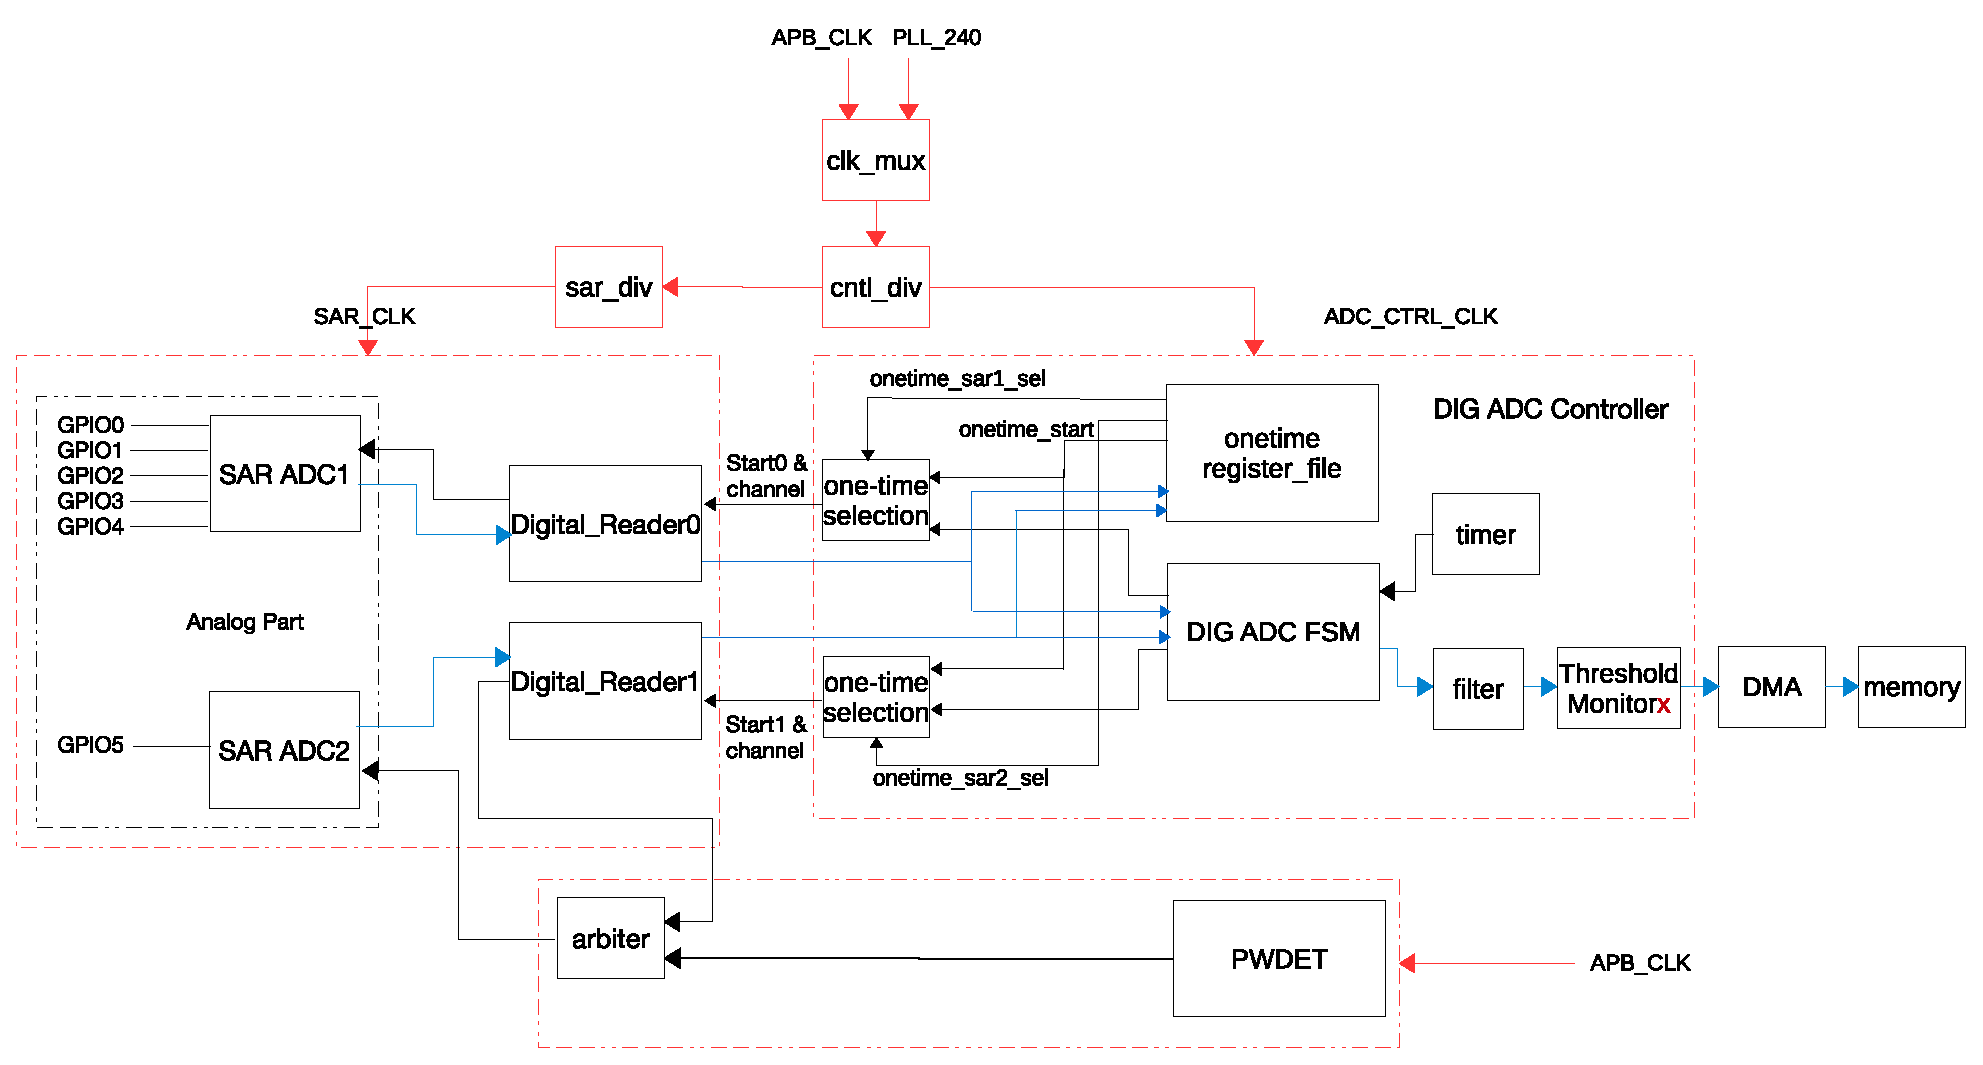
\includegraphics[width=1.1\textwidth]{./20-SENSOR/figures/on_chip_sensor_20240606}
    \textcolor{blue}{\textbf{——}}：数据流；\textcolor{red}{\textbf{——}}：时钟信号；\textcolor{black}{\textbf{——}}：控制信号
    \caption{SAR ADC 的功能概况}
    \label{fig:sensor-sar-adc-function-overview}
\end{figure}


如图 \ref{fig:sensor-sar-adc-function-overview} 所示，SAR ADC 模块主要包括以下元件：

\begin{itemize}
    \item SAR ADC1：可对五个通道进行电压检测；
    \item SAR ADC2：可对一个通道进行电压检测 
    \item 时钟管理：对时钟源进行选择和分频：
        \begin{itemize}
            \item 时钟源：可选择 APB\_CLK 或 PLL\_240；
            \item 分频时钟：
             \begin{itemize}
                 \item SAR\_CLK：SAR ADC1、SAR ADC2、Digital\_Reader0 和 Digital\_Reader1 的工作时钟；其中控制 SAR\_CLK 分频的 sar\_div 的分频系数至少是 2 分频；
                 \item ADC\_CTRL\_CLK：DIG ADC FSM 的工作时钟。
             \end{itemize}
        \end{itemize}
    \item 仲裁器 (arbiter)：用于选择使用 ADC2 的控制器，可以是 DIG ADC 控制器或 PWDET 控制器。
    \item \label{other:sensor-item-read-data-from-sar-adc1} Digital\_Reader0：由 DIG ADC FSM 驱动，读取 SAR ADC1 的数值；
    \item Digital\_Reader1：由 DIG ADC FSM 驱动，读取 SAR ADC2 的数值；
    \item DIG ADC FSM：生成整个 ADC 采样过程中所需的各种信号，下文简称 FSM。
    \item Threshold Monitor\regindex{x}：阈值监控器 1 和阈值监控器 2。可在采样值大于设定的高阈值，或小于设定的低阈值时触发中断。
\end{itemize}
以下小节将详细介绍各个元件。

\subsubsection{输入信号}

SAR ADC 需首先通过内部多路器选择待测量的模拟管脚，然后才能采样模拟信号。表 \ref{tab:sensor-sar-adc-input-signals} 列出了所有可能需要经过 SAR ADC1 或 SAR ADC2 处理的模拟信号。

\begin{longtable}{ |p{3cm}|p{1.5cm}|p{2cm}| }
    \caption{SAR ADC 的信号输入}
    \label{tab:sensor-sar-adc-input-signals}
    \\\hline
    \rowcolor{lightgray}
    信号名称 & 通道编号  & ADC 选择 \\\hline
    \endfirsthead
    \hline
    \rowcolor{lightgray}   
    信号名称 & 通道编号  & ADC 选择 \\\hline
    \endhead
    \hline
    \endfoot
    GPIO0       &  0  & \multirow{5}{*}{SAR ADC1} \\ \cline{1-2}
    GPIO1       &  1  & \\ \cline{1-2}
    GPIO2       &  2  & \\ \cline{1-2}
    GPIO3       &  3  & \\ \cline{1-2}
    GPIO4       &  4  & \\ \cline{1-3}
    GPIO5       &  0  & SAR ADC2 \\ \hline
\end{longtable}

\subsubsection{ADC 转换和衰减}

SAR ADC 转换模拟信号时，转换分辨率（12 位）电压范围为 0 mV \verb+~+ \(V_{ref}\)。其中，\(V_{ref}\) 为 SAR ADC 内部参考电压，出厂设定为 1100 mV。因此，转换结果 (data) 可以使用以下公式转换成模拟电压输出 \(V_{data}\)：

    \[
    V_{data} = \frac{V_{ref}}{k}\times{\frac{data}{4095}}
    \]

其中 \(k\) 为衰减对应的系数。

如需转换大于 \(V_{ref}\) 的电压，信号输入 SAR ADC 前可进行衰减。支持的衰减等级包括：

\begin{itemize}
    \item 0 dB (k≈100\%)
    \item 2.5 dB (k≈75\%)
    \item 6 dB (k≈50\%)
    \item 12 dB (k≈25\%)
\end{itemize}

\subsubsection{DIG ADC 控制器}


DIG ADC 控制器使用快速时钟，实现了采样速率大幅提升。该控制器最高支持 12 位采样分辨率，同时支持软件触发的单次采样和专用定时器触发的多通道扫描。更多参数和性能信息见\href{https://www.espressif.com/sites/default/files/documentation/esp32-c3_datasheet_en.pdf}{《ESP32-C3 系列芯片技术规格书》}中的 ADC 特性章节。

软件驱动的单次采样的具体配置如下：
\begin{itemize}
    \item 选择需要进行单次采样的 SAR ADC：
    \begin{itemize}
        \item 置位 APB\_SARADC1\_ONETIME\_SAMPLE 选择对 SAR ADC1 进行单次采样；
        \item 置位 APB\_SARADC2\_ONETIME\_SAMPLE 选择对 SAR ADC2 进行单次采样。
    \end{itemize}
    \item 配置 APB\_SARADC\_ONETIME\_CHANNEL 选择采样通道；
    \item 配置 APB\_SARADC\_ONETIME\_ATTEN 选择衰减；
    \item 配置 APB\_SARADC\_ONETIME\_START 启动单次采样；
    \item 采样结束即触发 APB\_SARADC\_ADC\regindex{x}\_DONE\_INT\_RAW 中断。软件检测该中断后，可在 APB\_SARADC\_AD\\C\regindex{x}\_DATA 寄存器内读到采样值。这里的 \regindex{x} 可以是 1 或 2。为 1 时表示 SAR ADC1；为 2 时表示 SAR ADC2。 
\end{itemize}

如果选择专用定时器驱动的多通道扫描，可采用如下配置。注，在多通道扫描模式下，扫描序列可根据样式表的描述进行，样式表可配置。 
\begin{itemize} 
        \item 配置 \hyperref[fielddesc:APBSARADCSARADCTIMERTARGET]{APB\_SARADC\_TIMER\_TARGET} 设置 DIG ADC 定时器的触发周期。当计数器计数到配置周期数的 2 倍时，触发采样。计数器的工作时钟见章节 \ref{other:sensor-para-dig-adc-clock}；
        \item 配置 \hyperref[fielddesc:APBSARADCSARADCTIMEREN]{APB\_SARADC\_TIMER\_EN} 使能定时器；
        \item 定时器超时则将驱动 DIG ADC FSM 根据样式表进行采样；
        \item 数据通过 DMA 自动存储到内存空间中，扫描完成将产生中断。
\end{itemize}

\begin{tiplisting}
单次采样不能和多通道扫描共用一个 SAR ADC。因此，当多通道扫描的样式表包含某个 SAR ADC 的采样指令时，该 SAR ADC 不能配置为单次采样。
\end{tiplisting}

\subsubsection{DIG ADC 时钟}\label{other:sensor-para-dig-adc-clock}

用户可配置 APB\_SARADC\_CLK\_SEL 选择 DIG ADC 控制器的工作时钟：
\begin{itemize}
    \item 1：选择 PLL\_240M 的分频时钟 ADC\_CTRL\_CLK；
    \item 0：选择 APB\_CLK。
\end{itemize}

如果选择使用 ADC\_CTRL\_CLK，用户可配置 APB\_SARADC\_CLKM\_DIV\_NUM 选择分频系数。注意，由于 SAR ADC 有速度限制，所以 Digital\_Reader0（包括 SAR ADC1）和 Digital\_Reader1（包括 SAR ADC2）的工作时钟是 SAR\_CLK，SAR\_CLK 频率会影响采样精度，频率越低采样精度越高。SAR\_CLK 由 ADC\_CTRL\_CLK 经过专用分频器分频所得。分频系数通过 APB\_SARADC\_SAR\_CLK\_DIV 配置。ADC 每采样一个数据需要 25 个 SAR\_CLK 时钟周期数，所以最大采样速率受到 SAR\_CLK 的频率限制。更多时钟信息，见章节 \ref{mod:resclk} \textit{\nameref{mod:resclk}}。

\subsubsection{DMA 支持}

DIG ADC 控制器允许通过外设 DMA 实现直接内存访问，由 DIG ADC 专用定时器产生触发信号。用户可通过软件配置 \hyperref[fielddesc:APBSARADCAPBADCTRANS]{APB\_SARADC\_APB\_ADC\_TRANS} 将 DMA 的数据通路切换到 DIG ADC。关于 DMA 的具体配置，请参考章节 \ref{mod:dma} \textit{\nameref{mod:dma}}。

\subsubsection{DIG ADC FSM}
\textbf{概述}

图 \ref{fig:sensor-diagram-dig-adc-fsm} 展示了 DIG ADC FSM 的工作原理。

\begin{figure}[H]
    \centering
    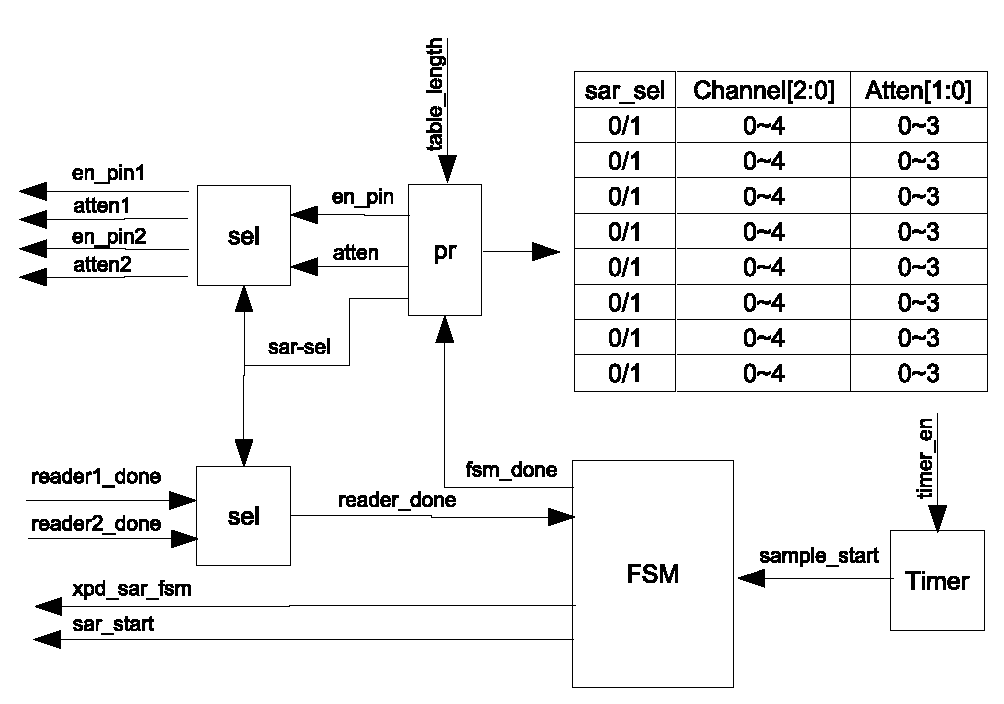
\includegraphics[width=0.7\textwidth]{./20-SENSOR/figures/20-sensor-saradc_dma_20210901}
    \caption{DIG ADC FSM 概况}
    \label{fig:sensor-diagram-dig-adc-fsm}
\end{figure}

其中，
\begin{itemize}
    \item Timer：表示 DIG ADC 的专用定时器，可产生 sample\_start 信号；
    \item pr：样式表指针，FSM 将根据该指针指向的样式配置，发送相应信号。
\end{itemize}

相关执行过程如下：
\begin{itemize}
\item 置位 \hyperref[fielddesc:APBSARADCSARADCTIMEREN]{APB\_SARADC\_TIMER\_EN} 使能 DIG ADC 的专用定时器。定时器超时将触发 sample\_start 信号驱动 FSM 模块开始采样；
\item FSM 模块收到 sample\_start 信号后，执行以下操作：
\begin{itemize}
    \item 开启 SAR ADC 电源；
    \item 根据当前 pr 指向的样式，选择 SAR ADC1 或 SAR ADC2 用作工作 ADC，同时配置 ADC 通道以及衰减；
    \item 根据配置信息，输出相应的 en\_pad（使能管脚）以及 atten（衰减）信号到模拟端；
    \item 发起 sar\_start 信号，开启采样。
\end{itemize}

    \item FSM 收到 ADC Reader（Digital\_Reader0 或 Digital\_Reader1）返回的 reader\_done 信号后，
    \begin{itemize}
        \item 结束采样；
        \item 将数据传输给滤波器 (filter)，然后阈值监控器 (threshold monitor) 通过 DMA 将数据传输给内存（见图 \ref{fig:sensor-sar-adc-function-overview}）；
        \item 更新样式表指针 pr，等待下一次采样。注意，如果指针 pr 小于 APB\_SARADC\_SAR\_PATT\_LEN (table\_length)，则 pr = pr + 1；否则 pr 将被清零。
    \end{itemize}
\end{itemize}    
    



\textbf{样式表结构}

DIG ADC FSM 包含一个样式表，由 APB\_SARADC\_SAR\_PATT\_TAB1\_REG 和 APB\_SARADC\_SAR\_PATT\_\\TAB2\_REG 两个寄存器组成，如图 \ref{fig:sensor-apb-saradc-sar-patt-tab1-reg-pattern-tab-entry0-entry3} 和图 \ref{fig:sensor-apb-saradc-sar-patt-tab2-reg-pattern-tab-entry4-entry7} 所示：

\regfield{(reserved)}{8}{24}{00000000}%
\regfield{cmd3}{6}{18}{{0x0000}}%
\regfield{cmd2}{6}{12}{{0x0000}}%
\regfield{cmd1}{6}{6}{{0x0000}}%
\regfield{cmd0}{6}{0}{{0x0000}}%
\begin{regdesc}\begin{reglist}
\item [cmd \regindex{x}] 表示样式表中的样式，即样式 0 \verb+~+ 样式 3。
\end{reglist}\end{regdesc}
\vspace{-2em}
\begin{figure}[H]
    \centering
    \caption{APB\_SARADC\_SAR\_PATT\_TAB1\_REG 与样式 0 - 3}
    \label{fig:sensor-apb-saradc-sar-patt-tab1-reg-pattern-tab-entry0-entry3}
\end{figure}

\regfield{(reserved)}{8}{24}{00000000}%
\regfield{cmd7}{6}{18}{{0x0000}}%
\regfield{cmd6}{6}{12}{{0x0000}}%
\regfield{cmd5}{6}{6}{{0x0000}}%
\regfield{cmd4}{6}{0}{{0x0000}}%
\begin{regdesc}\begin{reglist}
\item [cmd \regindex{x}] 表示样式表中的样式，即样式 4 \verb+~+ 样式 7。
\end{reglist}\end{regdesc}
\vspace{-2em}
\begin{figure}[H]
    \centering
    \caption{APB\_SARADC\_SAR\_PATT\_TAB2\_REG 与样式 4 - 7}
    \label{fig:sensor-apb-saradc-sar-patt-tab2-reg-pattern-tab-entry4-entry7}
\end{figure}

每个寄存器包含四个样式，每个样式长度为六位，共包括三个字段，分别存储了选择的工作 ADC、通道和衰减信息，具体见表 \ref{fig:sensor-pattern-table-entry}。

\begin{figure}[H]
\centering
\regfield{sar\_sel}{1}{5}{{x}}%
\regfield{ch\_sel}{3}{2}{{xx}}%
\regfield{atten}{2}{0}{xx}%
\end{figure}
\vspace{-2em}
\begin{figure}[H]
    \centering
    \caption{样式表中的样式结构}
    \label{fig:sensor-pattern-table-entry}
\end{figure}
\vspace{-2em}
\begin{regdesc}\begin{reglist}
\item [atten] 衰减配置信息。0：0 dB；1：2.5 dB；2：6 dB；3：12 dB。
\item [ch\_sel] 扫描通道选择信息，更多信息见表 \ref{tab:sensor-sar-adc-input-signals}。
\item [sar\_sel] ADC 选择信息。0：选择 SAR ADC1；1：选择 SAR ADC2。
\end{reglist}\end{regdesc}




\textbf{多通道扫描配置示例}

例如，希望实现如下所示的多通道扫描方式：
\begin{itemize}
    \item 扫描 SAR ADC1 的通道 2，且衰减配置为 12 dB；
    \item 扫描 SAR ADC2 的通道 0，且衰减配置为 2.5 dB。
\end{itemize}

则具体的配置如下：
\begin{itemize}
    \item 配置第一个样式 cmd0，如下图所示：

\centering
\regfield{sar\_sel}{1}{5}{{0}}%
\regfield{ch\_sel}{3}{2}{{2}}%
\regfield{atten}{2}{0}{3}%
\reglabel{}\regnewline%
\begin{regdesc}\begin{reglist}
\begin{figure}[H]
    \centering
    \caption{cmd0 配置示例}
\end{figure}
\vspace{-2em}
\item [atten] 配置该字段的值为 3，即衰减配置为 12 dB。
\item [ch\_sel] 配置该字段的值为 2，即选择通道 2（见表 \ref{tab:sensor-sar-adc-input-signals}）。
\item [sar\_sel] 配置该位为 0，即选择 SAR ADC1。
\end{reglist}\end{regdesc}
\end{itemize}

\begin{itemize}
    \item 配置第二个样式 cmd1，如下图所示：

\centering
\regfield{sar\_sel}{1}{5}{{1}}%
\regfield{ch\_sel}{3}{2}{{0}}%
\regfield{atten}{2}{0}{1}%
\reglabel{}\regnewline%
\begin{regdesc}\begin{reglist}
\begin{figure}[H]
    \centering
    \caption{cmd1 配置示例}
\end{figure}
\vspace{-2em}
\item [atten] 配置该字段的值为 1，即衰减配置为 2.5 dB。 
\item [ch\_sel] 配置该字段的值为 0，即选择通道 0（见表 \ref{tab:sensor-sar-adc-input-signals}）。
\item [sar\_sel] 配置该位为 1，即选择 SAR ADC2。
\end{reglist}\end{regdesc}
\end{itemize}

\begin{itemize}
    \item 配置 APB\_SARADC\_SAR\_PATT\_LEN 为 1，即选择使用上述配置好的样式表 0 和样式表 1；
    \item 使能定时器，则 DIG ADC 控制器将根据上述样式配置，周期性采样 SAR ADC1 的通道 2 和 SAR ADC2 的通道 0。
\end{itemize}

\textbf{DMA 数据格式}

ADC 最终向 DMA 传递 32 位数据，如下图所示：

\begin{figure}[H]
\centering
\regfield{reserved}{15}{17}{{xx}}%
\regfield{sar\_sel}{1}{16}{{x}}%
\regfield{ch\_sel}{3}{13}{{xxx}}%
\regfield{reserved}{1}{12}{{x}}%
\regfield{data}{12}{0}{xx}%
\end{figure}
\vspace{-2em}
\begin{figure}[H]
    \centering
    \caption{DMA 数据格式}
    \label{fig:sensor-dma-data-format}
\end{figure}
\vspace{-2em}
\begin{regdesc}\begin{reglist}
\item [data] ADC 转换结果，12 位
\item [ch\_sel] 通道信息，3 位
\item [sar\_sel] ADC 选择信息，1 位
\end{reglist}\end{regdesc}





\subsubsection{ADC 滤波器}
DIG ADC 控制器支持滤波功能，提供两个滤波器。两个滤波器均可配置给任一 SAR ADC 的任一通道，然后对目标通道的采样数据进行滤波。滤波公式如下所示：

\[data_{cur} = \frac{(k-1)data_{prev}}{k}+\frac{data_{in}}{k}+0.5\]

\begin{itemize}
    \item \(data_{cur}\)：滤波后数据
    \item \(data_{in}\)：ADC 采样值
    \item \(data_{prev}\)：上次滤波数据
    \item \(k\)：滤波系数
\end{itemize}

配置滤波器如下：
\begin{itemize}
\item 配置 APB\_SARADC\_FILTER\_CHANNEL\regindex{x} 设置滤波器 \regindex{x} 作用的 ADC 通道
\item 配置 APB\_SARADC\_FILTER\_FACTOR\regindex{x} 设置滤波器 \regindex{x} 的滤波系数
\end{itemize}

注意，这里的 \regindex{x} 为滤波器编号：\regindex{x} 为 0 表示滤波器 \regindex{0}；为 1 表示滤波器 \regindex{1}。

\subsubsection{阈值监控}
DIG ADC 包含两个阈值监控器，可配置到 SAR ADC1 和 SAR ADC2 的任意通道上。当 ADC 采样值大于设定的高阈值，则触发高阈值中断；若采样值小于设定的低阈值，则触发低阈值中断。

阈值监控配置如下：
\begin{itemize}
    \item 配置 APB\_SARADC\_THRES\regindex{x}\_EN 使能阈值监控 \regindex{x} 的功能；
    \item 配置 APB\_SARADC\_THRES\regindex{x}\_LOW 设置低阈值；
    \item 配置 APB\_SARADC\_THRES\regindex{x}\_HIGH 设置高阈值；
    \item 配置 APB\_SARADC\_THRES\regindex{x}\_CHANNEL 设置监控的 SAR ADC 以及通道。
\end{itemize}

注意，这里的 \regindex{x} 为阈值监控器编号：\regindex{x} 为 0 表示阈值监控器 \regindex{0}；为 1 表示阈值监控器 \regindex{1}。

\subsubsection{SAR ADC2 仲裁器}

SAR ADC2 可选两种控制器：DIG ADC 控制器或 PWDET 控制器。为防止出现冲突，同时提升 SAR ADC2 的使用效率，\chipname{} 提供了 SAR ADC2 的访问仲裁。仲裁器有公平仲裁和固定优先级仲裁两种模式可供选择。

\begin{itemize}
    \item 公平仲裁模式，即循环优先级仲裁。清零 \hyperref[fielddesc:APBSARADCADCARBFIXPRIORITY]{APB\_SARADC\_ADC\_ARB\_FIX\_PRIORITY} 位即可进入公平仲裁模式。
    \item 固定优先级仲裁模式下，配置 \hyperref[fielddesc:APBSARADCADCARBAPBPRIORITY]{APB\_SARADC\_ADC\_ARB\_APB\_PRIORITY} 位 (DIG ADC 控制器) 和 \hyperref[fielddesc:APBSARADCADCARBWIFIPRIORITY]{APB\_\\SARADC\_ADC\_ARB\_WIFI\_PRIORITY} 位 (PWDET 控制器) 
   可分别配置对应控制器的优先级。值越大，优先级越高。
\end{itemize}


仲裁器规定，无论低优先级控制器是否已开始转换数据，高优先级控制器均可随时开始自己的数据转换。如果 ADC 已经接受低优先级控制器的转换请求，开始转换数据，但高优先级控制器也需要转换数据，则可以中断或终止低优先级控制器的数据转换，开始高优先级控制器的数据转换。如果已经有高优先级控制器正在进行数据转换，而低优先级控制器则无法启动数据转换。

转换中断或转换启动失败返回的转换数据无效，因此在返回的转换结果中增加数据标记位，表示转换是否有效。

\begin{itemize}
    \item DIG ADC 控制器的数据标记位为 DMA 数据类型的 \{sar\_sel, ch\_sel[2:0]\} 位，见图 \ref{fig:sensor-dma-data-format}
    \begin{itemize}
        \item 4'b1111：数据转换中断
        \item 4'b1110：数据转换启动失败
        \item 对应的通道号：转换数据有效
    \end{itemize}
    \item PWDET 控制器的数据标记位为采样结果的高两位
    
    \begin{itemize}
        \item 2'b10：数据转换中断
        \item 2'b01：数据转换启动失败
        \item 2'b00：转换数据有效
    \end{itemize}
\end{itemize}
除了上述两种模式以外，用户可以通过配置 \hyperref[fielddesc:APBSARADCADCARBGRANTFORCE]{APB\_SARADC\_ADC\_ARB\_GRANT\_FORCE} 屏蔽仲裁器，配置 \hyperref[fielddesc:APBSARADCADCARBWIFIFORCE]{APB\_\\SARADC\_ADC\_ARB\_WIFI\_FORCE} 或 \hyperref[fielddesc:APBSARADCADCARBAPBFORCE]{APB\_SARADC\_ADC\_ARB\_APB\_FORCE} 决定授权控制器。

\section{温度传感器}\label{sec:sensor-temp-sensor}
\subsection{概述}
\chipname{} 搭载了温度传感器可以实时监测芯片内部温度。
\subsection{特性} 
温度传感器的主要特性包括：
\begin{itemize}
    \item 支持软件触发，且一旦触发后，可持续读取数据
    \item 可根据使用环境配置温度偏移，提高测试精度
    \item 测量范围可调节
\end{itemize}


\subsection{功能描述}

温度传感器可由软件启动，具体配置如下：
    \begin{itemize}
        \item 置位 \hyperref[fielddesc:APBSARADCTSENSPU]{APB\_SARADC\_TSENS\_PU}，温度传感器上电；
        \item 置位 \hyperref[fielddesc:SYSTEMTSENSCLKEN]{SYSTEM\_TSENS\_CLK\_EN} 使能温度传感器时钟；
        \item 等待 \hyperref[fielddesc:APBSARADCTSENSXPDWAIT]{APB\_SARADC\_TSENS\_XPD\_WAIT} 个时钟周期后，温度传感器的复位释放，开始测量环境温度；
        \item 等待一段时间后（输出值会随着测量时间的增加而逐渐线性逼近真实的温度值），直接从 \hyperref[fielddesc:APBSARADCTSENSOUT]{APB\_SARADC\_TSENS\_OUT} 中即可持续获取温度值。
    \end{itemize}



温度传感器的输出值需要使用转换公式转换成实际的温度值(°C)。转换公式如下： 
\[
        T(°C) = 0.4386 * VALUE – 27.88 * offset – 20.52
\]


其中 VALUE 即温度传感器的输出值，offset 由温度偏移决定。 温度传感器在不同的实际使用环境（测量温度范围）下，温度偏移不同，见表 \ref{tab:tsensor-dac}。


\begin{longtable}[c]{|p{4cm}|p{4cm}|}
    \caption{温度传感器的温度偏移}
    \label{tab:tsensor-dac}
    \\\hline
    \rowcolor{lightgray}
    测量范围 (°C)  & 温度偏移 (°C) \\\hline
    50 \verb+~+ 125 & -2 \\\hline
    20 \verb+~+ 100 & -1 \\\hline
    -10 \verb+~+ 80 & 0 \\\hline
    -30 \verb+~+ 50 & 1 \\\hline
    -40 \verb+~+ 20 & 2 \\\hline
\end{longtable}

\section{中断}

\begin{itemize}
   \item \label{interreupt:SARADCDONEINT1} APB\_SARADC\_ADC1\_DONE\_INT：SAR ADC1 完成一次转换，即触发此中断；
   \item \label{interreupt:SARADCDONEINT2} APB\_SARADC\_ADC2\_DONE\_INT：SAR ADC2 完成一次转换，即触发此中断；
   \item \label{interreupt:APBSARADCTHRESxHIGHINT} APB\_SARADC\_THRES\regindex{x}\_HIGH\_INT：超过阈值监控器 \regindex{x} 的高阈值，即触发此中断；
    \item \label{interreupt:APBSARADCTHRESxLOWINT} APB\_SARADC\_THRES\regindex{x}\_LOW\_INT：低于阈值监控器 \regindex{x} 的低阈值，即触发此中断。
\end{itemize}



\section{寄存器列表}



本小节的所有地址均为相对于 ADC 控制器基地址的地址偏移量（相对地址），具体基地址请见章节 \ref{mod:sysmem} \textit{\nameref{mod:sysmem}} 中的表 \ref{tab:sysmem-base-address}。

请查看章节 \hyperref[glossary-access-types]{\textit{寄存器的访问类型}}，了解“访问”列缩写的含义。

\subfile{\modulefiles/apb_saradc_sw_pass_reg_summary_20210409}

\section{寄存器}

本小节的所有地址均为相对于 ADC 控制器基地址的地址偏移量（相对地址），具体基地址请见章节 \ref{mod:sysmem} \textit{\nameref{mod:sysmem}} 中的表 \ref{tab:sysmem-base-address}。

\subfile{\modulefiles/apb_saradc_sw_pass_reg_20210409}

\end{document}
